% Gemini theme
% Adapted for the EEGxPlore FACED poster draft.

\documentclass[final]{beamer}

% ====================
% Packages
% ====================

\usepackage[T1]{fontenc}
\usepackage{lmodern}
\usepackage[size=custom,width=121.92,height=91.44,scale=1.0]{beamerposter}
\usetheme{gemini}
\usecolortheme{gemini}
\usepackage{graphicx}
\usepackage{booktabs}
\usepackage{tikz}
\usepackage{pgfplots}
\pgfplotsset{compat=1.14}
\graphicspath{{../figure/}}

% ====================
% Lengths
% ====================

% Three-column 36" x 48" poster:
% (N+1)*\sepwidth + N*\colwidth = \paperwidth
\newlength{\sepwidth}
\newlength{\colwidth}
\setlength{\sepwidth}{0.025\paperwidth}
\setlength{\colwidth}{0.30\paperwidth}

\newcommand{\separatorcolumn}{\begin{column}{\sepwidth}\end{column}}

\newcommand{\placeholder}[2]{%
  \begin{center}
    \fbox{%
      \parbox[c][#1][c]{0.94\linewidth}{%
        \centering
        \Large #2
      }%
    }
  \end{center}
}

\newcommand{\metricrow}[4]{#1 & #2 & #3 & #4 \\}

% ====================
% Title
% ====================

\title{Selective Beats Broad: Late, Depth-Aware Sparse Adaptation on FACED}

\author{[Author 1] \inst{1} \and [Author 2] \inst{1} \and [Author 3] \inst{1}}

\institute[shortinst]{\inst{1} [Lab / Department / University]}

% ====================
% Footer
% ====================

\footercontent{
  EEGxPlore poster draft \hfill
  Downstream adaptation on pretrained CBraMod \hfill
  [contact email]}

% ====================
% Logo
% ====================

\logoright{\includegraphics[height=6.5cm]{CBraMod_logo.png}}

% ====================
% Body
% ====================

\begin{document}

\begin{frame}[t]
\begin{columns}[t]
\separatorcolumn

\begin{column}{\colwidth}

  \begin{alertblock}{Takeaway}
    \small
    The best observed FACED result came from a small, targeted intervention:
    \textbf{pre-attention depth summaries + one late typed MoE layer + MLP
    routing + a 15-dim summary}. This poster studies \textbf{downstream
    adaptation on top of pretrained CBraMod}; it is \textbf{not} a new EEG
    foundation-model pretraining paper.
  \end{alertblock}

  \begin{block}{Main Contribution}
    \small
    We propose a \textbf{downstream adaptation recipe} on top of pretrained
    CBraMod. The central result is that \textbf{selective, late, depth-aware
    sparse adaptation} outperformed broader specialization on FACED, suggesting
    a practical adaptation strategy for EEG foundation models.
  \end{block}

  \begin{block}{Background / Motivation}
    \small
    EEG foundation models can transfer strong general representations, but
    downstream EEG adaptation is still difficult because subject-specific
    variability remains large, supervision is limited, and the same decoder has
    to stay reliable across heterogeneous recordings. Sparse routing is
    attractive in this setting because it can specialize parts of the model
    without fully retraining the backbone. But broader specialization is not
    automatically better: more modified paths, more expert layers, or larger
    routing signals can increase optimization difficulty and sometimes reduce
    robustness instead of improving it.

    \vspace{0.4cm}
    We therefore ask a narrower question:
    \textbf{what is the smallest effective sparse adaptation strategy for a
    pretrained EEG foundation model?}
  \end{block}

  \begin{block}{Question}
    \small
    Can \textbf{depth-use patterns} act as a compact routing signal that helps
    downstream specialization \textbf{without broad modification of the
    backbone}?
  \end{block}

  \begin{block}{Method Overview}
    \small
    Our best recipe keeps the pretrained \textbf{CBraMod} backbone largely
    intact and adds only a late sparse specialization step.

    \vspace{0.3cm}
    \begin{itemize}
      \item The backbone first produces \textbf{pre-attention depth-use /
      AttnRes summaries} that capture how information is being selected across
      depth.
      \item Those depth-use signals are compressed into a \textbf{compact router
      context} rather than exposing the router to a broad, high-dimensional
      state.
      \item That compact context guides \textbf{one late typed MoE layer} near
      the end of the encoder.
      \item The MoE uses separate \textbf{spatial} and \textbf{spectral} expert
      banks so the two feature families do not have to share identical routing.
      \item Routing stabilization is kept concise: soft dispatch, entropy /
      balance regularization, jitter annealing, and warmup.
    \end{itemize}
  \end{block}

  \begin{block}{Figure 1: Method Overview}
    \small
    \placeholder{17cm}{Figure 1 placeholder\\[0.5em]
    Pretrained CBraMod backbone $\rightarrow$ pre-attention depth summary
    $\rightarrow$ compact router context $\rightarrow$ one late typed MoE layer
    with spatial and spectral expert banks}

    \vspace{0.3cm}
    One clean pipeline figure is enough here; the text block above already
    explains the moving parts.
  \end{block}

\end{column}

\separatorcolumn

\begin{column}{\colwidth}

  \begin{block}{Main Result on FACED}
    \small
    The strongest observed FACED configuration was \textbf{selective rather
    than broad}: \texttt{pre\_attn} placement, \texttt{1} late MoE layer,
    \texttt{mlp} routing, and a compact \texttt{15}-dim summary. It improved
    on the conservative sparse baseline and also exceeded broader alternatives
    such as \texttt{full} backbone modification and two MoE layers.

    \vspace{0.3cm}
    Relative to the best conservative sparse baseline, the best selective run
    improved test balanced accuracy by \textbf{+0.02174}, Cohen's
    $\kappa$ by \textbf{+0.02446}, and weighted F1 by \textbf{+0.02346}.
  \end{block}

  \begin{block}{Figure 2: Main Result Comparison}
    \small
    \begin{center}
      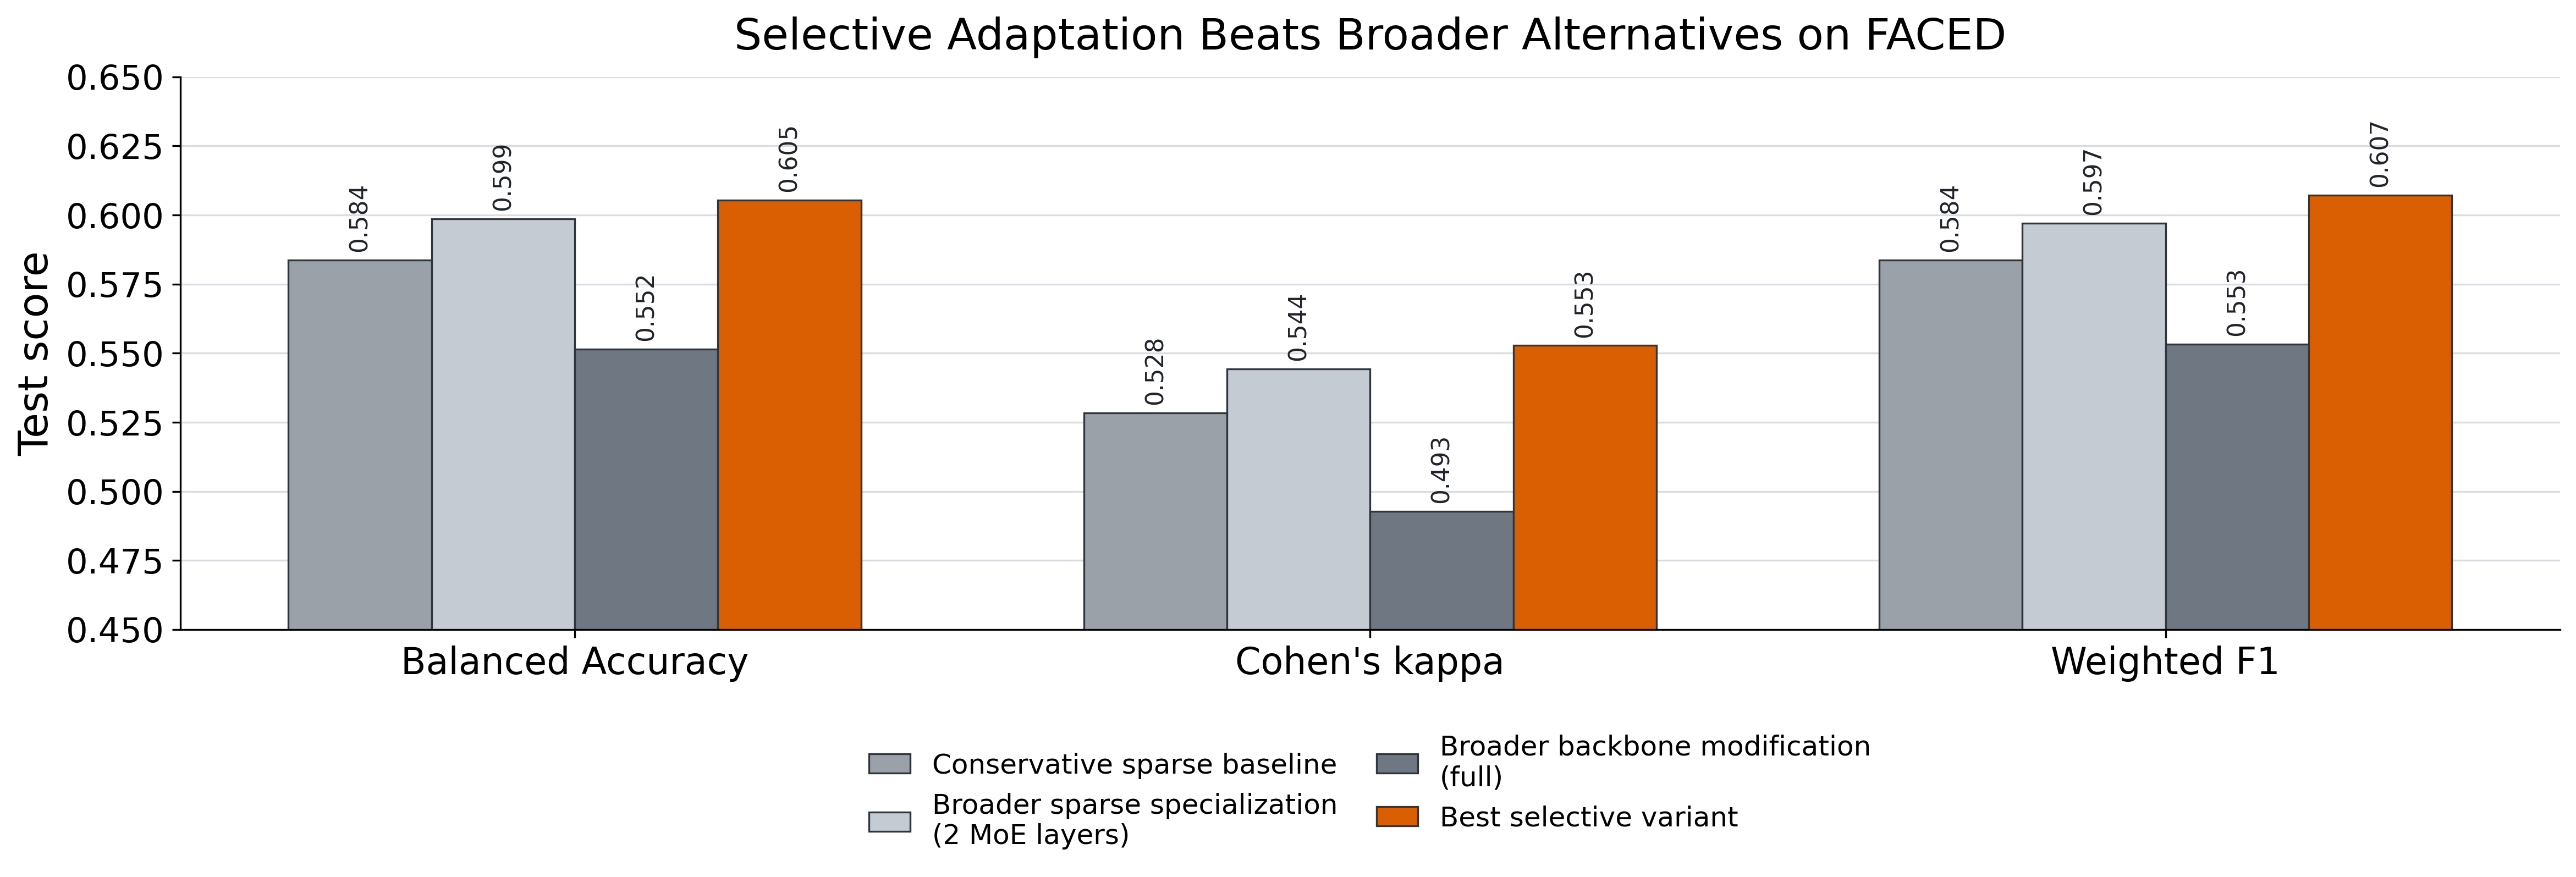
\includegraphics[width=0.94\linewidth]{faced_main_results.pdf}
    \end{center}

    \vspace{0.1cm}
    Neutral tones show the broader or baseline alternatives; the accent color
    marks the best selective variant.
  \end{block}

  \begin{block}{FACED Comparison with Prior Foundation-Model Baselines}
    \scriptsize
    \begin{tabular}{p{0.34\linewidth} r r r}
      \toprule
      \textbf{Model} & \textbf{Acc.} & \textbf{$\kappa$} & \textbf{F1} \\
      \midrule
      EEGConformer & 0.4156 & 0.3270 & 0.4044 \\
      BIOT & 0.4870 & 0.4215 & 0.4865 \\
      LaBraM-Base & 0.5211 & 0.4586 & 0.5300 \\
      CBraMod & 0.5509 & 0.5041 & 0.5618 \\
      \textbf{Ours (best selective adaptation)} & \textbf{0.6055} & \textbf{0.5528} & \textbf{0.6072} \\
      \bottomrule
    \end{tabular}

    \vspace{0.2cm}
    Cross-paper FACED comparisons may differ by protocol or split and are
    shown for context only. Prior baseline values are taken from Table 2 of
    the CBraMod paper.
  \end{block}

  \begin{exampleblock}{Setup + Best Current Configuration}
    \small
    \textbf{Setup}
    \begin{itemize}
      \item Backbone: pretrained CBraMod
      \item Dataset: FACED
      \item Evaluation: subject-disjoint train / validation / test
      \item Metrics: balanced accuracy, Cohen's $\kappa$, weighted F1
    \end{itemize}

    \vspace{0.1cm}
    \textbf{Best verified configuration}
    \begin{itemize}
      \item Placement: \texttt{pre\_attn}
      \item Sparse depth: \texttt{1} late typed MoE layer
      \item Router: \texttt{mlp}
      \item Summary: \texttt{15}-dim \texttt{attn\_delta4}
      \item Router context: MLP depth probe enabled
    \end{itemize}

    \vspace{0.1cm}
    \textbf{Best validation checkpoint}: 0.62515 balanced accuracy, 0.57716
    $\kappa$, 0.63056 weighted F1

    \vspace{0.1cm}
    \textbf{Test}: 0.60548 balanced accuracy, 0.55276 $\kappa$, 0.60721
    weighted F1
  \end{exampleblock}

\end{column}

\separatorcolumn

\begin{column}{\colwidth}

  \begin{block}{Figure 3: Key Ablation Results}
    \scriptsize
    \textbf{Main ablations}

    \vspace{0.15cm}
    \begin{tabular}{p{0.34\linewidth} r r r p{0.26\linewidth}}
      \toprule
      \textbf{Variant} & \textbf{Acc.} & \textbf{$\kappa$} & \textbf{F1} & \textbf{Interpretation} \\
      \midrule
      Pretrained / dense baseline* & 0.586 & 0.529 & 0.586 & Separate no-MoE FACED branch; use cautiously \\
      Conservative sparse MoE baseline & 0.584 & 0.528 & 0.584 & Stable sparse reference \\
      \texttt{pre\_attn} (best selective) & 0.605 & 0.553 & 0.607 & Best observed FACED result \\
      \texttt{full} (best) & 0.552 & 0.493 & 0.553 & Broader backbone change underperformed \\
      1 MoE layer (best) & 0.605 & 0.553 & 0.607 & Best sparse depth \\
      2 MoE layers (best) & 0.599 & 0.544 & 0.597 & Broader specialization did not win \\
      Linear router (best) & 0.599 & 0.546 & 0.601 & Close, but below MLP \\
      MLP router (best) & 0.605 & 0.553 & 0.607 & Best routing choice \\
      \bottomrule
    \end{tabular}

    \vspace{0.45cm}
    \textbf{Summary-size / content ablations}

    \vspace{0.15cm}
    \begin{tabular}{p{0.34\linewidth} r r r p{0.26\linewidth}}
      \toprule
      \textbf{Variant} & \textbf{Acc.} & \textbf{$\kappa$} & \textbf{F1} & \textbf{Interpretation} \\
      \midrule
      Summary dim 11 & 0.589 & 0.533 & 0.590 & Too small to match best selective run \\
      Summary dim 13 & 0.582 & 0.528 & 0.584 & Below dim 15 \\
      Summary dim 15 & 0.605 & 0.553 & 0.607 & Best compact summary size \\
      Summary dim 26 & 0.116 & 0.007 & 0.050 & Verified collapse in observed run \\
      \texttt{attn\_delta4} + probe & 0.605 & 0.553 & 0.607 & Best summary recipe \\
      \texttt{attn\_delta4} no probe & 0.604 & 0.552 & 0.606 & Probe helped slightly \\
      \texttt{attn\_mlp\_balanced} & 0.596 & 0.542 & 0.597 & Worse than \texttt{attn\_delta4} \\
      \texttt{attn\_mlp\_latemix} & 0.588 & 0.532 & 0.588 & Worst of controlled content sweep \\
      \bottomrule
    \end{tabular}

    \vspace{0.25cm}
    *Dense baseline row comes from an older no-MoE FACED run in the sibling
    CBraMod log tree, not from the current typed-MoE sweep.
  \end{block}

  \begin{alertblock}{What This Poster Does And Does Not Claim}
    \small
    \begin{itemize}
      \item This is a \textbf{downstream adaptation} result on top of pretrained
      CBraMod.
      \item Evidence here is strongest on \textbf{FACED} only.
      \item We do \textbf{not} claim a new pretraining method.
      \item We do \textbf{not} claim cross-dataset generality yet.
      \item Cross-paper comparisons should remain secondary because splits and
      protocols differ.
    \end{itemize}
  \end{alertblock}

  \begin{block}{Why Might Selective Work?}
    \small
    The strongest FACED runs suggest that downstream adaptation benefited more
    from \textbf{late, compact, depth-aware specialization} than from broader
    intervention. A plausible interpretation is that the router only needs a
    small amount of backbone-state information to make useful specialization
    decisions, while broader modification adds optimization burden without
    guaranteed benefit. The routing exports do show that spatial and spectral
    expert usage are not identical, but those diagnostics are more useful as a
    cautious interpretation than as a central poster figure.
  \end{block}

  \begin{block}{Next Steps}
    \small
    \begin{itemize}
      \item Test whether the same selective recipe transfers to additional EEG
      datasets
      \item Add per-subject variance and uncertainty summaries
      \item Refine the content of the compact depth summary
      \item Better characterize what spatial vs spectral experts are capturing
    \end{itemize}
  \end{block}

  \begin{block}{References / Notes}
    \small
    \begin{itemize}
      \item CBraMod: Criss-Cross Brain Foundation Model for EEG Decoding
      \item FACED dataset paper
      \item AttnRes reference
      \item Sparse / MoE adaptation references
    \end{itemize}
  \end{block}

\end{column}

\separatorcolumn
\end{columns}
\end{frame}

\end{document}
